\section{First Model}

\subsection{Deriving the ODE for the rainbowfish population}

\begin{flushleft}
    An Ordinary Differential Equation needs to model the rainbow fish population change.
    The growth rate of the rainbowfish population is 70\% with
    a maximum aquarium capacity of 750 fishes. The death rate is
    estimated to be 0.001 because one fish lives for 1000
    days, therefore the odds of a fish dying is 0.001, which is then
    multiplied by the number of fishes. $0.001P(t)$
    However this is negligible and is
    removed since the decrease it makes is really small.
    However, 20 rainbowfishes are sold every day,
    so that's included in the model and is not negligible.
\end{flushleft}

\begin{equation}
    \frac{dP}{dt} = 0.7P(t)(1-\frac{P(t)}{750})-20
\end{equation}

\subsection{Results from numerical solution in Python}
\begin{flushleft}

    The model was then solved numerically in Python using
    euler's formula with timestep $\Delta t=\frac{1}{16}$
    which gave the following results:

\end{flushleft}

\begin{figure}[H]
    \centering
    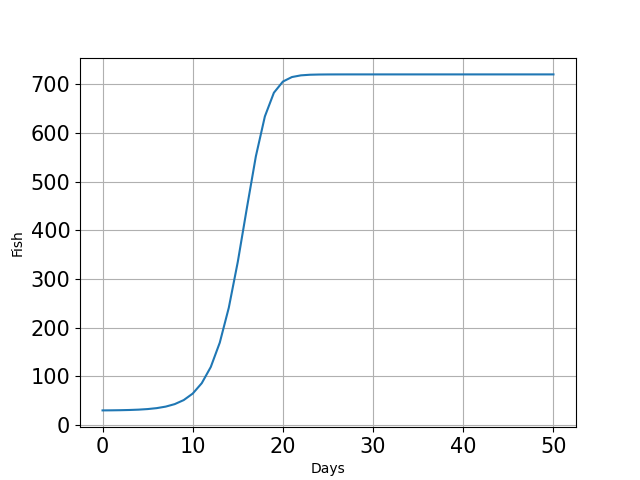
\includegraphics[scale=0.4]{../figures/Figure_1.png}
    \caption{The number of rainbowfish over time with $P(0)=20$}
\end{figure}

\begin{flushleft}
    As we can see, the amount of rainbowfish approaches somewhere
    above 700.
    The exact amount is 720.2, but since you can not have
    fractional fish we can approximate it to 720. This is
    a stable equilibrium point as the population would decrease if it went up and increase if it was lowered.
\end{flushleft}

\begin{flushleft}
    As a conclusion this model does work for one fish,
    however we want to introduce a second type of fish
    into the model. The gourami.
\end{flushleft}